\chapter{Joint Entropy}

\section{Multivariate Distributions}

\subsection{Partitioning the Sample Space}
A random variable \( X \) can be viewed as a partition of the sample space \( \Omega \), where each outcome in \( \Omega \) is associated with a specific value of \( X \). This partitions \( \Omega \) into disjoint subsets corresponding to different values of \( X \).

\begin{marginfigure}
    \includegraphics[width=1\textwidth]{img/partition.png}
    \caption{Recall the definition of a random variable as a function from the sample space $\Omega$. We can think of this as a partition of the set $\Omega$.}
\end{marginfigure}


\subsection{Joint Random Variables}
When considering joint random variables \( X \) and \( Y \), these can be thought of as creating different partitions of the same sample space \( \Omega \). The joint probability \( p(X = x, Y = y) \) represents the intersection of the preimages of \( x \) and \( y \), which is the probability of both events happening simultaneously:
\[
    p(X = x, Y = y) = p(\omega \in X^{-1}(x) \cap Y^{-1}(y)).
\]

\begin{center}
    \includegraphics[width=1\textwidth]{img/joint_partition.png}
\end{center}

\ex{Joint Distributions on a Die}{Consider a die, with sample space \( \Omega = \{1, 2, 3, 4, 5, 6\} \). Define two random variables \( X \) and \( Y \):
    \begin{itemize}
        \item \( X \): whether the number rolled is even.
        \item \( Y \): whether the number rolled is greater than 3.
    \end{itemize}


    \begin{center}
        \begin{tabular}{ccc}
            \toprule
            \( \omega \) & \( X(\omega) \) & \( Y(\omega) \) \\
            \midrule
            1            & 0               & 0               \\
            2            & 1               & 0               \\
            3            & 0               & 0               \\
            4            & 1               & 1               \\
            5            & 0               & 1               \\
            6            & 1               & 1               \\
            \bottomrule
        \end{tabular}
    \end{center}

}


\subsection{Marginal and Conditional Probabilities}
The marginal probability \( p(X = x) \) gives the probability of \( X = x \) regardless of \( Y \):
\[
    p(X = x) = \sum_{y \in Y} p(X = x, Y = y).
\]
The conditional probability \( p(X = x | Y = y) \) is the probability of \( X = x \) given that \( Y = y \) has occurred:
\[
    p(X = x | Y = y) = \frac{p(X = x, Y = y)}{p(Y = y)}.
\]

\sn{Conditioning on Impossible Events}{If \( p(Y = y) = 0 \), then \( p(X | Y = y) \) is undefined.}

\subsection{Joint Probability Rules}

Joint probabilities satisfy several fundamental rules:

\begin{itemize}
    \item \textbf{Product Rule:} The probability of the joint occurrence of \( X \) and \( Y \) can be factored as:
          \[
              p(X = x, Y = y) = p(X = x | Y = y) p(Y = y).
          \]

    \item \textbf{Sum Rule:} The marginal probability of \( X = x \) can be derived by summing over all possible values of \( Y \):
          \[
              p(X = x) = \sum_{y \in Y} p(X = x | Y = y) p(Y = y).
          \]

    \item \textbf{Bayes' Theorem:} This rule relates conditional probabilities by switching the conditioning:
          \[
              p(X = x | Y = y) = \frac{p(Y = y | X = x) p(X = x)}{p(Y = y)}.
          \]
    \item The same intuitions apply in continous spaces, with integrals replacing sums.
\end{itemize}

\sn{Warning: Notation Overload}{
    \raggedright
    The symbol \( p \) in expressions like \( p(x) \) and \( p(y) \) technically represents different functions for each variable. For clarity, the precise way to write this would be  \( p_X(X = x) \) or \( p_Y(Y = y) \), though we often simplify to \( p(x) \) when it is unambigious from the context.}

\subsection{Statistical Independence}

\defb{Independent Random Variables}{
    A set of random variables \( \{X_1, X_2, \ldots, X_n\} \) is independent if, for any subset \( \{X_{i_1}, X_{i_2}, \ldots, X_{i_k}\} \),
    \[
        p(X_{i_1}, X_{i_2}, \ldots, X_{i_k}) = p(X_{i_1}) p(X_{i_2}) \cdots p(X_{i_k}).
    \]
    For \( n = 2 \), we denote this as \( X_1 \perp\!\!\!\perp X_2 \), which implies that \( p(X_1 | X_2) = p(X_1) \).
}

We distinguish two types of independence:

\begin{itemize}
    \item \textbf{Marginal Independence:} Two random variables \( X \) and \( Y \) are independent if \( p(X, Y) = p(X) p(Y) \).
    \item \textbf{Conditional Independence:} Given a third variable \( Z \), \( X \) and \( Y \) are conditionally independent if \( p(X, Y | Z) = p(X | Z) p(Y | Z) \), denoted as \( X \perp\!\!\!\perp Y | Z \).
\end{itemize}

\sn{Warning: Conditional Independence}{
    Conditioning on a variable can create or destroy dependence. \bigskip

    \textbf{Example of Creating Independence }
    \begin{itemize}
        \item \( X \) represents whether a person carries an umbrella.
        \item \( Y \) represents whether the ground is wet.
        \item Let \( Z \) represent the weather, sunny or rainy.
    \end{itemize}

    $X$ and $Y$ are dependent because seeing someone with an umbrella makes it more likely that the ground is wet because it's raining. However, if we know the weather, i.e. conditioning on $Z$, then $X$ and $Y$ are independent– given it is raining, knowing the fact of whether a person carries an umbrella no longer provides any additional information about whether the ground is wet.\bigskip

    \textbf{Example of Destroying Independence}
    \begin{itemize}
        \item \( X \) is the outcome of Coin A (heads or tails).
        \item \( Y \) is the outcome of Coin B (heads or tails).
        \item Let \( Z \) whether the coins show the same outcome (heads-heads or tails-tails).
    \end{itemize}
    Say you flip Coin A and Coin B, you know $X$ and $Y$ are independent as the result of one coin flip does not affect the other. However, conditioning on $Z$ (i.e. knowing the coins show the same outcome) destroys this independence. If you know the coins show the same outcome, then the outcome of Coin A tells you the outcome of Coin B, and vice versa.

}


\marginnote{
    \ex{Conditional Independence Example}{
        Let \( f \) and \( g \) be stochastic functions. If \( Y = f(X) \) and \( Z = g(Y) \), then \( X \) and \( Z \) are dependent (\( X \not\perp\!\!\!\perp Z \)) but become conditionally independent given \( Y \), i.e., \( X \perp\!\!\!\perp Z | Y \). \bigskip

        As another example, if \( X \) and \( Y \) are independent fair coin flips (i.e., \( X, Y \sim B(0.5) \)), and \( Z = (X + Y) \mod 2 \), then \( X \) and \( Z \) are independent but become dependent when conditioned on \( Y \).
    }}

\section{Graphical Models}

\defb{Bayesian Network}{
    A \textbf{Bayesian network} is a directed network where each node represents a random variable (RV), and the edges represent a factorisation of the joint probability density function (PDF). Formally, given a set of random variables \( X = \{X_1, X_2, \dots, X_k\} \), the joint distribution is factorised as:
    \[
        p(X) = \prod_{k} p(X_k | \text{pa}(X_k))
    \]
    where \(\text{pa}(X_k)\) denotes the set of parents of \(X_k\). In this representation, the directed edges indicate conditional dependencies among variables.
}

\begin{figure}[h]
    \centering
    % Improved Bayesian Network Diagram
    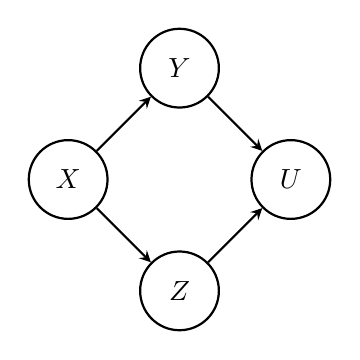
\begin{tikzpicture}[->, >=stealth, node distance=2cm, thick]
        \node[circle, draw, minimum size=1cm](X) {\(X\)};
        \node[circle, draw, minimum size=1cm, above right of=X](Y) {\(Y\)};
        \node[circle, draw, minimum size=1cm, below right of=X](Z) {\(Z\)};
        \node[circle, draw, minimum size=1cm, below right of=Y](U) {\(U\)};

        \draw[->] (X) -- (Y);
        \draw[->] (X) -- (Z);
        \draw[->] (Y) -- (U);
        \draw[->] (Z) -- (U);
    \end{tikzpicture}
    \caption{Bayesian Network example}
\end{figure}

This network represents the joint probability factorisation:
\[
    p(X, Y, Z, U) = p(X) p(Y|X) p(Z|X) p(U|Y,Z)
\]

\section{Markov Chains and Joint Entropy}

\defb{Markov Chain}{
    A stochastic process \( X_1, X_2, \dots, X_n \) is called a \textbf{Markov chain} if, for all \( t \),
    \[
        p(X_t | X_{t-1}, X_{t-2}, \dots, X_1) = p(X_t | X_{t-1})
    \]
    In other words, each state \( X_t \) depends only on the previous state \( X_{t-1} \), not on earlier states. This is often denoted as \( X_1 \to X_2 \to \dots \to X_n \).
}

% Markov Chain Diagram
\begin{figure}[h]
    \centering
    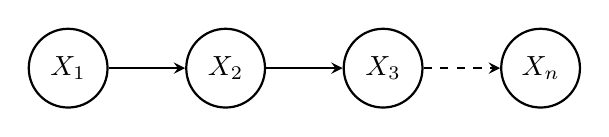
\begin{tikzpicture}[->, >=stealth, node distance=2cm, thick]
        \node[circle, draw, minimum size=1cm](X1) {\(X_1\)};
        \node[circle, draw, minimum size=1cm, right of=X1](X2) {\(X_2\)};
        \node[circle, draw, minimum size=1cm, right of=X2](X3) {\(X_3\)};
        \node[circle, draw, minimum size=1cm, right of=X3](X4) {\(X_n\)};

        \draw[->] (X1) -- (X2);
        \draw[->] (X2) -- (X3);
        \draw[dashed, ->] (X3) -- (X4);
    \end{tikzpicture}
    \caption{Markov Chain Diagram}
\end{figure}

The above diagram illustrates a simple Markov chain, where each variable depends only on the preceding variable. In writing, we also consider Markov chains of order $p$:

\[p(X_t | X_{t-1}, X_{t-2}, \cdots, X_1) = p(X_t | X_{t-1}, \cdots, X_{t-p})\]

\defb{Joint Entropy}{
    The \textbf{joint entropy} of two random variables \( X \) and \( Y \), with alphabets \( \mathcal{X} \) and \( \mathcal{Y} \), is defined as:
    \[
        H(X, Y) = - \sum_{x \in \mathcal{X}} \sum_{y \in \mathcal{Y}} p(x, y) \log p(x, y)
    \]
    Joint entropy represents the combined uncertainty in predicting both \( X \) and \( Y \) simultaneously. It is symmetric, so \( H(X, Y) = H(Y, X) \).
}

All properties of entropy apply to joint entropy.
\begin{itemize}
    \item Expected value of joint surprisal, $\mathbb{E}_p[-\log p(X, Y)]$, is the joint entropy.
    \item Uncertainty when predicting $X$ and $Y$ jointly.
    \item Minimum code length when encoding $X$ and $Y$ simultaneously.
\end{itemize}

\defb{Conditional Entropy}{
    The \textbf{conditional entropy} of \( X \) given \( Y \), denoted \( H(X|Y) \), represents the uncertainty in \( X \) when \( Y \) is known. It is given by:
    \[
        H(X|Y) = \sum_{y \in \mathcal{Y}} p(y) H(X|Y = y)
    \]
    where
    \[
        H(X|Y = y) = - \sum_{x \in \mathcal{X}} p(x|y) \log p(x|y)
    \]
    Conditional entropy quantifies the remaining uncertainty in \( X \) after observing \( Y \). \bigskip

    Note that $H(X|Y)$ is not defined when $p(Y = y) = 0$ for any $y$. To fix this, we either sum over $y$ such that $p(Y = y) > 0$ or use the limit definition of entropy, where $\frac{0}{0} \log 0 = 0$.
}


Some important properties of conditional entropy for discrete random variables:

\begin{itemize}
    \item \textbf{Non-negativity:} \( H(X|Y) \geq 0 \).

          \textbf{Proof:} Since probabilities \( p(x|y) \leq 1 \), we have \( -\log p(x|y) \geq 0 \). Thus, each term in the summation is non-negative, ensuring \( H(X|Y) \geq 0 \).

    \item \textbf{Upper Bound:} \( H(X|Y) \leq \log |\mathcal{X}| \), where \( |\mathcal{X}| \) is the size of the alphabet of \( X \).

          \textbf{Proof:} This follows similarly to the upper bound on \( H(X) \), using the fact that \( -\log p(x|y) \leq \log |\mathcal{X}| \) for all \( x \).

    \item \textbf{Deterministic Dependency:} \( H(X|Y) = 0 \) if \( X \) is a deterministic function of \( Y \).

          \textbf{Proof:} If \( X \) is completely determined by \( Y \), then \( p(x|y) \) is either \( 1 \) or \( 0 \) for each \( x \) given \( y \), making \( -\log p(x|y) = 0 \) wherever \( p(x|y) = 1 \).

    \item \textbf{Independence:} If \( X \) and \( Y \) are independent, then \( H(X|Y) = H(X) \).

          \textbf{Proof:} Independence implies \( p(x|y) = p(x) \), and so:
          \[
              H(X|Y = y) = - \sum_{x \in \mathcal{X}}p(x|y)\log p(x|y)= - \sum_{x \in \mathcal{X}} p(x) \log p(x) = H(X).
          \]
          Averaging over \( y \) yields \( H(X|Y) = H(X).\)
\end{itemize}

\subsection{Conditional Kullback-Leibler (KL) Divergence}

\defb{Conditional KL Divergence}{
    The \textbf{conditional Kullback-Leibler (KL) divergence} between two conditional probability distributions \( p(X|Y) \) and \( q(X|Y) \) is defined as:
    \[
        D_{\text{KL}}(p(X|Y) \parallel q(X|Y)) = \sum_{y \in \mathcal{Y}} p(y) D_{\text{KL}}(p(X|Y = y) \parallel q(X|Y = y)),
    \]
    where
    \[
        D_{\text{KL}}(p(X|Y = y) \parallel q(X|Y = y)) = \sum_{x \in \mathcal{X}} p(x|y) \log \frac{p(x|y)}{q(x|y)}.
    \]
}

\begin{itemize}
    \item \textbf{Non-negativity:} \( D_{\text{KL}}(p(X|Y) \parallel q(X|Y)) \geq 0 \).

          \textbf{Explanation:}
          The non-negativity follows from the non-negativity of each individual term \( D_{\text{KL}}(p(X|Y = y) \parallel q(X|Y = y)) \), as each conditional KL divergence is non-negative.

    \item \textbf{Zero Value:} \( D_{\text{KL}}(p(X|Y) \parallel q(X|Y)) = 0 \) if and only if \( p(X|Y) = q(X|Y) \) for all \( y \).

          \textbf{Explanation:}
          This holds because each \( D_{\text{KL}}(p(X|Y = y) \parallel q(X|Y = y)) = 0 \) if and only if \( p(x|y) = q(x|y) \) for all \( x \) and \( y \), meaning the two distributions are identical.

    \item \textbf{Additivity:} For independent conditional distributions, \( D_{\text{KL}}(p(X,Y) \parallel q(X,Y)) = D_{\text{KL}}(p(X|Y) \parallel q(X|Y)) + D_{\text{KL}}(p(Y) \parallel q(Y)) \).

          \textbf{Explanation:}
          This property arises because the joint divergence \( D_{\text{KL}}(p(X,Y) \parallel q(X,Y)) \) can be decomposed into divergences over conditional and marginal components when \( p(X|Y) \) and \( q(X|Y) \) are conditionally independent.
\end{itemize}


\ex{Joint and Conditional Entropy Example}{
    Consider random variables \( X \) and \( Y \) with the following probability distribution:

    \begin{center}
        \begin{tabular}{c|cc|c}
            \( p(x, y) \) & \( x = 0 \)       & \( x = 1 \)       & \( p(y) \)        \\
            \hline
            \( y = 0 \)   & \( \frac{1}{8} \) & \( 0 \)           & \( \frac{1}{8} \) \\
            \( y = 1 \)   & \( \frac{1}{8} \) & \( \frac{1}{4} \) & \( \frac{3}{8} \) \\
            \( y = 2 \)   & \( \frac{1}{4} \) & \( \frac{1}{4} \) & \( \frac{1}{2} \) \\
            \hline
            \( p(x) \)    & \( \frac{1}{2} \) & \( \frac{1}{2} \) &                   \\
        \end{tabular}
    \end{center}

    Calculating the entropies for this distribution:

    \begin{itemize}
        \item \( H(X) = 1 \) bit
        \item \( H(Y) = 1.41 \) bits
        \item \( H(X|Y) = 0.84 \) bits
        \item \( H(Y|X) = 1.25 \) bits
        \item \( H(X, Y) = 2.25 \) bits
    \end{itemize}

    This example illustrates how joint and conditional entropies quantify the combined and remaining uncertainties within a pair of random variables.
}

\subsection{Entropy Chain Rule}

\thm{Entropy Chain Rule}{
    For two random variables \( X \) and \( Y \), the entropy chain rule states:
    \[
        H(X, Y) = H(X | Y) + H(Y)
    \]
    This is a foundational property in information theory, allowing the joint entropy \( H(X, Y) \) to be decomposed into the sum of the conditional entropy \( H(X | Y) \) and the marginal entropy \( H(Y) \).


    \paragraph{Proof:}
    Starting with the definition of joint entropy:
    \[
        H(X, Y) = - \sum_{x, y} p(x, y) \log p(x, y)
    \]

    we can rewrite \( p(x, y) \) in terms of the conditional and marginal distributions:
    \[
        = - \sum_{x, y} p(x | y) p(y) \log (p(x | y) p(y))
    \]

    Expanding the logarithm gives:
    \[
        = - \sum_{x, y} p(x | y) p(y) \left( \log p(x | y) + \log p(y) \right)
    \]

    Now we distribute \( p(x | y) p(y) \) across the sum:
    \[
        = - \sum_{x, y} p(x | y) p(y) \log p(x | y) - \sum_{x, y} p(x | y) p(y) \log p(y)
    \]

    The first term simplifies to the conditional entropy \( H(X | Y) \):
    \[
        = H(X | Y) - \sum_{y} p(y) \log p(y) \underbrace{\sum_{x} p(x | y)}_{= 1}
    \]

    Since \( \sum_{x} p(x | y) = 1 \) for each \( y \), the second term becomes:
    \[
        = H(X | Y) - \sum_{y} p(y) \log p(y) \cancel{\underbrace{\sum_{x} p(x | y)}_{1}}
    \]

    This simplifies further to:
    \[
        H(X,Y) = H(X | Y) + H(Y)
    \]
    which proves the chain rule.
}

\subsection{Invariance of Entropy under Isomorphisms}


\defb{Isomorphisms of RVs}{
    Two random variables \( X \) and \( Y \) are said to be \textbf{isomorphic} if there exists a bijective (one-to-one and onto) function \( f \) such that:
    \[
        X = f(Y) \quad \text{and} \quad Y = f^{-1}(X)
    \]
    This implies that \( X \) and \( Y \) can be perfectly mapped to each other without any loss of information. Therefore, the uncertainty (entropy) of \( X \) is exactly the same as that of \( Y \).
}

\begin{marginfigure}
    \centering
    \resizebox{1\linewidth}{!}{ % Adjust 0.8\linewidth to scale as desired
        \begin{tikzpicture}[ele/.style={fill=black,circle,minimum width=.8pt,inner sep=1pt, scale=0.5},every fit/.style={ellipse,draw,inner sep=-2pt}]
            \node[ele,label=left:$a$] (a1) at (0,4) {};
            \node[ele,label=left:$b$] (a2) at (0,3) {};
            \node[ele,label=left:$c$] (a3) at (0,2) {};
            \node[ele,label=left:$d$] (a4) at (0,1) {};

            \node[ele,label=right:$1$] (b1) at (4,4) {};
            \node[ele,label=right:$2$] (b2) at (4,3) {};
            \node[ele,label=right:$3$] (b3) at (4,2) {};
            \node[ele,label=right:$4$] (b4) at (4,1) {};

            \node[draw,fit= (a1) (a2) (a3) (a4),minimum width=2cm] {} ;
            \node[draw,fit= (b1) (b2) (b3) (b4),minimum width=2cm] {} ;
            \draw[->,thick,shorten <=2pt,shorten >=2pt] (a1) -- (b4);
            \draw[->,thick,shorten <=2pt,shorten >=2pt] (a2) -- (b2);
            \draw[->,thick,shorten <=2pt,shorten >=2pt] (a3) -- (b1);
            \draw[->,thick,shorten <=2pt,shorten >=2pt] (a4) -- (b3);
        \end{tikzpicture}
    }
    \caption{Visualisation of a bijective function between two sets of random variables.}
\end{marginfigure}

\thm{Invariance of Entropy}{
    Entropy is invariant under isomorphisms of discrete random variables. Specifically, if two random variables \( X \) and \( Y \) are isomorphic, then \( H(X) = H(Y) \).


    \paragraph{Proof:}
    We can demonstrate this by applying the entropy chain rule in both directions:
    \[
        H(X, Y) = H(X) + H(Y | X) = H(Y) + H(X | Y)
    \]

    Since \( X = f(Y) \), knowing \( Y \) completely determines \( X \), meaning \( H(X | Y) = 0 \). Similarly, \( Y = f^{-1}(X) \) implies \( H(Y | X) = 0 \).

    Thus, we have:
    \[
        H(X) = H(Y)
    \]
    which confirms that the entropy of \( X \) is equal to the entropy of \( Y \) when they are isomorphic.
}

\section{Stochastic Processes}

Previously, we covered the case of two RVs, $X$ and $Y$, but can extend this to $n$ joint RVs with stochastic processes.

\defb{Stochastic Process}{
A \textbf{stochastic process} is a collection of random variables indexed by time (or another ordering parameter). Formally, a stochastic process is represented as \( \{X_i\}_{i \in T} \), where \( T \) is the index set, and each \( X_i \) is a random variable. Here, we will consider semi-infinite processes \( \{X_1, X_2, \dots, X_n\} \).
}

\defb{Stationary Stochastic Process}{
    A stochastic process is \textbf{stationary} if its statistical properties are invariant to shifts in time. For a stationary process, the joint distribution of any subset of variables is the same, regardless of the starting point. \bigskip

    Formally, a stochastic process has, for all \( t \) and \( s \):
    \[
        p(X_1, X_2, \dots, X_t) = p(X_{1+s}, X_{2+s}, \dots, X_{t+s})
    \]
    In essence, time shifts do not alter the distribution.
}

\subsection{Entropy Rate and Innovation}

\defb{Entropy Rate}{
    Refers to how quickly \( H(X_1, X_2, \dots, X_n) \) grows as \( n \) becomes large. \bigskip

    The \textbf{entropy rate} of a stochastic process measures the asymptotic growth rate of the joint entropy \( H(X_1, X_2, \dots, X_n) \) as \( n \) becomes large. For a stationary process \( \{X_i\} \), the entropy rate \( h(X) \) is defined as:
    \[
        h_1(X) = \lim_{n \to \infty} \frac{1}{n} H(X_1, X_2, \dots, X_n)
    \]
}

\defb{Innovation}{
    Refers to how much new information is introduced at time $n$. \bigskip

    \textbf{Innovation} quantifies the amount of new information introduced by each new observation in a stochastic process. It is defined as the conditional entropy of the next observation given all past observations:
    \[
        h_2(X) = \lim_{n \to \infty} H(X_n | X_1, X_2, \dots, X_{n-1})
    \]
}

\thm{Entropy Rate Theorem}{
    For a stationary stochastic process, the entropy rate and the innovation rate are equal:
    \[
        h(X) = \lim_{n \to \infty} \frac{1}{n} H(X_1, X_2, \dots, X_n) = \lim_{n \to \infty} H(X_n | X_1, X_2, \dots, X_{n-1})
    \]
    This result provides a way to measure the information growth in a stationary process by either the average entropy per observation or the amount of new information introduced at each step.
}
\newpage
\marginnote[8.5pt]{
    \thm{Cesaro Mean}{
        \raggedright
        The Cesaro Mean Theorem states, if $a_n \to a$, and $b_n = \frac{1}{n} \sum_{i=1}^n a_i$, then $b_n \to a$. \label{thm:cesaro} \bigskip

        Since $a_n \to a$, there exists a number $N(\epsilon)$ such that for all $n \geq N(\epsilon)$, $|a_n - a| < \epsilon$. Hence,
        \begin{align*}
            \left| b_n - a \right| & = \left| \frac{1}{n} \sum_{i=1}^{n} (a_i - a) \right|                       \\
                                   & \leq \frac{1}{n} \sum_{i=1}^{n} \left| a_i - a \right|                      \\
                                   & \leq \frac{1}{n} \sum_{i=1}^{N(\epsilon)} \left| a_i - a \right| +          \\ &  \quad \frac{n - N(\epsilon)}{n} \epsilon  \\
                                   & \leq \frac{1}{n} \sum_{i=1}^{N(\epsilon)} \left| a_i - a \right| + \epsilon
        \end{align*}

        For all \( n \geq N(\epsilon) \). Since the first term goes to 0 as \( n \to \infty \), we can make \( |b_n - a| \leq 2\epsilon \) by taking \( n \) large enough. Hence \( b_n \to a \) as \( n \to \infty \). \(\qed\)



    }
}
\extrab{Proof of the Entropy Rate Theorem}{

    See Cover \& Thomas (1991) Theorem 4.2.1. We want to show
    \[
        h(X) = \underbrace{\lim_{n \to \infty} \frac{1}{n} H(X_1, X_2, \dots, X_n)}_{h_1(X)} = \underbrace{\lim_{n \to \infty} H(X_n | X_1, X_2, \dots, X_{n-1})}_{h_2(X)}
    \]



    We first show that the $h_2(X)$ limit exists, that the sequence of conditional entropies is a decreasing sequence. We have:
    \begin{align}
        H(X_{n+1}| X_1, X_2, \dots, X_n) & \leq H(X_{n+1} | X_n, X_{n-1}, \dots, X_2)                                    \\&= H(X_n| X_{n-1}, \dots, X_2, X_1) \label{eq:equality_stationarity} \\
        % \\
        % \Rightarrow h_2(X)               & \leq H(X_n| X_{n-1}, \dots, X_2, X_1)                                         \\
        \Rightarrow h_2(X)               & = \lim_{n \to \infty}  H(X_n| X_{n-1}, \dots, X_2, X_1) \label{eq:innovation}
    \end{align}

    where the inequality follows from the fact that conditioning on more variables reduces entropy. The first equality in \ref{eq:equality_stationarity} follows from the stationarity of the process (Markov). For \ref{eq:innovation}, since $H(X_n| X_{n-1}, \dots, X_2, X_1)$ is a decreasing sequence of nonnegative numbers, it has a limit which is the innovation rate. \bigskip



    By the chain rule,
    \[
        H(X_1, X_2) = H(X_1 | X_2) + H(X_2)
    \]
    We can then extend this to \( H(X_1, X_2, X_3) \) as:
    \begin{align*}
        H(X_1, X_2, X_3) & = H(X_1 | X_2, X_3) + H(X_2, X_3)         \\
                         & = H(X_1 | X_2, X_3) +  H(X_2 | X_3) + X_3
    \end{align*}

    The general formula is:

    \begin{equation}
        H(X_1, X_2, \dots X_n) = \sum_{i=1}^n H(X_i | X_{i-1}, X_{i-2}, \dots, X_1)
    \end{equation}
    i.e,the entropy rate is the time average of the conditional entropies. From the Cesaro Mean Theorem, we have
    \begin{align*}
        \frac{1}{n}H(X_1, X_2, \dots X_n)                     & = \frac{1}{n} \sum_{i=1}^n H(X_i | X_{i-1}, X_{i-2}, \dots, X_1)                     \\
        \lim_{n \to \infty} \frac{1}{n}H(X_1, X_2, \dots X_n) & = \lim_{n \to \infty} \frac{1}{n} \sum_{i=1}^n H(X_i | X_{i-1}, X_{i-2}, \dots, X_1) \\
                                                              & = \lim_{n \to \infty} H(X_n | X_{n-1}, \dots, X_2, X_1)
        = h_2(X)\end{align*}


    The running average has a limit, equal to the innovation rate $h_2(X)$ of the terms. This proves the equivalence of $h_1(X)$ and $h_2(X)$, and the entropy rate theorem.

    \[
        h_1(x) = \lim_{n \to \infty} \frac{1}{n}H(X_1, X_2, \dots, X_n) = \lim_{n \to \infty} H(X_n| X_{n-1}, \dots, X_2, X_1) = h_2(X)
    \] \hfill \(\blacksquare\)

}
\newpage
\section{Stochastic Processes}
\[
    H(X_{n+1} | X_1, \dots, X_n) \leq H(X_n | X_1, \dots, X_{n-1})
\]
\begin{itemize}
    \item When conditioning on no prior information (i.e., \( t = 0 \)), we have the full entropy \( H(X_n) \).
    \item As we condition on more previous observations, the conditional entropy decreases.
    \item Intuitively, $X$ is a time series, and $H(X_n | X_1, \dots, X_{n-1})$ is the performance of a predictor with $t$ timesteps of `memory'. Without memory $(t=0)$, we get usual entropy $H(X_n)$, with no memory of the past.
    \item Including more memory decreases the conditional entropy, as the predictor can use past observations to improve predictions. Eventually, the predictor reaches the entropy rate, where no further improvement is possible.
    \item If this happens at some finite $t = p$, the process is said to have a Markov order of $p$.
\end{itemize}

\begin{marginfigure}
    \includegraphics[width=\linewidth]{img/conditioning.png}
    \caption{In this diagram, we see that as the conditioning memory \( t \) increases, the conditional entropy \( H(X_n | X_{n-t}, \dots, X_{n-1}) \) decreases, eventually reaching the entropy rate \( h(X) \).}
\end{marginfigure}

\egb{Coin in a Box}{
    \textbf{Question:} What is the entropy rate of the following process?

    \begin{itemize}
        \item At \( t = 0 \), we flip a fair coin and place it in a box.
        \item At each subsequent time step \( t \), we shake the box, so the coin changes sides with probability \( p \).
    \end{itemize}

    \tcblower
    \textbf{Answer:} The entropy rate of this process as \( n \to \infty \) is given by:
    \begin{align*}
        \lim_{n \to \infty} \frac{1}{n} H(X_1, X_2, \dots, X_n) & = \lim_{n \to \infty} H(X_n | X_1, X_2, \dots, X_{n-1}) \\
                                                                & = H(X_{t+1} | X_t)                                      \\
                                                                & = H_2(p)
    \end{align*}
    where \( H_2(p) \) denotes the entropy of a biased coin with parameter \( p \).
}

\begin{itemize}
    \item The entropy rate measures the average amount of new information introduced by each step in a process.
    \item Useful for applications like compressing sequential data (e.g., language).
    \item "Stream codes," such as the Lempel-Ziv algorithm (used in compression formats like ZIP), are practical applications of entropy rates in stochastic processes.
\end{itemize}

\section{Mutual Information}

\defb{Mutual Information}{
    The mutual information between two random variables \( X \) and \( Y \) is defined as:
    \[
        I(X;Y) := \sum_{x,y \in \mathcal{X} \times \mathcal{Y}} p(x, y) \log \frac{p(x, y)}{p(x)p(y)}.
    \]
    This quantity, often denoted \( I(X; Y) \), measures the reduction in uncertainty of \( X \) given knowledge of \( Y \) (or vice versa).
    \begin{itemize}
        \item Mutual information is symmetric: \( I(X; Y) = I(Y; X) \).
        \item To separate the arguments in mutual information (MI), we use a semicolon (;) rather than a comma (,) for separating RVs, e.g., \( I(X; Y) \).
        \item In physics and some other fields, the arguments in mutual information are separated by a colon (:), so \( I(X: Y) \) may also be used.
    \end{itemize}
}



Mutual information can also be expressed as a difference in entropies:
\[
    I(X; Y) = H(X) + H(Y) - H(X, Y).
\]
Using the entropy chain rule, this can be further decomposed as:
\[
    I(X; Y) = \underbrace{H(X)}_{\text{Uncertainty about } X}- \underbrace{H(X | Y)}_{\text{uncertainty about } X \text{ given } Y}
\]
where \( I(X; Y) \) represents the average reduction in uncertainty about \( X \) given \( Y \).
\begin{itemize}
    \item Mutual information cannot exceed the minimum entropy of the two variables: \( I(X; Y) \leq \min \{ H(X), H(Y) \} \).
\end{itemize}


\subsection{Mutual Information as KL Divergence}
Mutual information can be interpreted as the Kullback-Leibler (KL) divergence between the joint probability distribution \( p(X, Y) \) and the product of the marginal distributions \( p(X)p(Y) \):
\begin{equation}
    I(X; Y) = D_{KL}(p(X, Y) \parallel p(X)p(Y)). \label{eq:mi_kl}
\end{equation}

\marginnote[-70pt]{
    Equation \ref{eq:mi_kl} implies two very important key properties:
    \begin{itemize}
        \item \textbf{Non-negativity}: Since KL divergence is always non-negative, mutual information \( I(X; Y) \geq 0 \).
        \item \textbf{Zero MI for Independence}: Mutual information is zero if and only if \( X \) and \( Y \) are independent, i.e., \( p(X, Y) = p(X)p(Y) \).

              This is because the KL divergence between two identical distributions is zero.


              $D_{KL}(p(X, Y) \parallel p(X)p(Y)) = 0 \Leftrightarrow p(X, Y) = p(X)p(Y)$.
    \end{itemize}}


\thm{Information Doesn’t Hurt}{
    For any two random variables \( X \) and \( Y \), conditioning on \( Y \) reduces the entropy of \( X \):
    \[
        H(X | Y) \leq H(X).
    \]


    \paragraph{Proof: }
    This result follows from the definition of mutual information:
    \[
        H(X) - H(X | Y) = I(X; Y) \geq 0,
    \]
    since mutual information \( I(X; Y) \) is always non-negative. Hence,
    \[
        H(X | Y) \leq H(X).
    \]
}

\begin{itemize}
    \item For continuous random variables, this inequality holds even though \( H(X) \) and \( H(X | Y) \) can individually be negative.
    \item In general, the conditional entropy \( H(X | Y = y) \) can sometimes exceed \( H(X) \), depending on the specific values of \( Y = y \).
\end{itemize}

\subsection{Conditional Mutual Information}
\marginnote{Since conditional mutual information can be viewed as a KL divergence, it has the following properties:
    \begin{itemize}
        \item \textbf{Non-negativity}: \( I(X; Y | Z) \geq 0 \).
        \item \textbf{Zero Condition}: \( I(X; Y | Z) = 0 \) if and only if \( X \) and \( Y \) are conditionally independent given \( Z \) (denoted \( X \perp\!\!\!\perp Y | Z \)).
    \end{itemize}}
\defb{Conditional Mutual Information}{
    The conditional mutual information (CMI) between random variables \( X \) and \( Y \) given \( Z \) is defined as:
    \[
        I(X; Y | Z) := \sum_{x, y, z \in \mathcal{X} \times \mathcal{Y} \times \mathcal{Z}} p(x, y, z) \log \frac{p(x, y | z)}{p(x | z) p(y | z)}.
    \]
    Conditional mutual information quantifies the amount of information shared between \( X \) and \( Y \) when conditioned on a third variable \( Z \).

    \begin{itemize}
        \item We can rewrite the CMI in terms of conditional entropies:
              \begin{align*}
                  I(X; Y | Z) & = H(X | Z) + H(Y | Z) - H(X, Y | Z) \\
                              & = H(X | Z) - H(X | Y, Z)
              \end{align*}

        \item CMI is a KL divergence:
              \[
                  I(X; Y | Z) = D_{\text{KL}}(p(X, Y | Z) \parallel p(X | Z)p(Y | Z))
              \]
    \end{itemize}

}





\section{Chain Rule for Mutual Information}

\thm{Mutual Information Chain Rule}{
    The chain rule for mutual information states that for any three random variables \( X \), \( Y \), and \( Z \):
    \[
        I(X, Y; Z) = I(X; Z) + I(Y; Z | X).
    \]

    That is, the mutual information between \( X \) and \( Y \) given \( Z \) can be decomposed into the mutual information between \( X \) and \( Z \) and the conditional mutual information between \( Y \) and \( Z \) given \( X \).

    \paragraph{Proof:}
    The proof of the chain rule follows from the properties of joint and conditional entropy:
    \[
        I(X, Y; Z) = H(X, Y) - H(X, Y | Z).
    \]
    Applying the chain rule for entropy, we can expand \( H(X, Y) \) and \( H(X, Y | Z) \). We rearrange and simplify:
    \begin{align}
        I(X, Y; Z) & = H(X, Y) - H(X, Y | Z)                                                                      \\
                   & = H(Y | X) + H(X) - \left( H(Y | X, Z) + H(X | Z) \right) \label{eq:mi_entropy_chain_rule}   \\
                   & = \underbrace{H(X) - H(X | Z)}_{I(X; Z)} + \underbrace{H(Y | X) - H(Y | X, Z)}_{I(Y; Z | X)} \\
                   & = I(X; Z) + I(Y; Z | X).
    \end{align}

    where the second equality follows from the entropy chain rule (see Equation~\ref{eq:mi_entropy_chain_rule}).

}


\pagebreak
\section{Mutual Information Invariance}
\marginnote[11pt]{\thm{Data Processing Inequality (DPI)}{
        If \( X \), \( Y \), and \( Z \) form a Markov chain \( X \to Y \to Z \), then:
        \[
            I(X; Z) \leq I(X; Y).
        \]
        \paragraph{Proof:}
        \begin{itemize}
            \item Applying the MI chain rule in both directions:
                  \begin{align*}
                       & I(X; Y, Z)              \\
                       & = I(X; Z) + I(X; Y | Z) \\
                       & = I(X; Y) + I(X; Z | Y)
                  \end{align*}

            \item By the definition of a Markov chain, \( X \perp\!\!\!\perp Z | Y \), and thus \( I(X; Z | Y) = 0 \).

            \item By the non-negativity of conditional mutual information (CMI), \( I(X; Y | Z) \geq 0 \). Thus,
                  \[
                      I(X; Z) \leq I(X; Y).
                  \]
        \end{itemize}
    }}

\marginnote{
    \sn{Note on Continuous Variables}{
        This invariance property also holds for continuous random variables, even though entropy terms such as \( H(X) \) and \( H(X | Y) \) may not themselves be invariant.
    }
}
\thm{Invariance of Mutual Information}{
    Mutual information \( I(X; Y) \) is invariant under bijective (one-to-one and onto) transformations of \( X \) or \( Y \).

    \paragraph{Proof:}

    Let \( V = f(Y) \), where \( f \) is a bijective function. This gives a new variable \( V \) that preserves all information in \( Y \). Since \( X \), \( Y \), and \( V \) form a Markov chain \( X \to Y \to V \), we can apply the \textbf{Data Processing Inequality (DPI)}:
    \[
        I(X; V) \leq I(X; Y).
    \]

    Similarly, because \( f \) is bijective, there exists an inverse \( f^{-1} \) such that \( Y = f^{-1}(V) \). This reverses the dependency chain, making \( X \to V \to Y \) a valid Markov chain, and by DPI, we have:
    \[
        I(X; Y) \leq I(X; V).
    \]

    Combining these two inequalities, we obtain:
    \[
        I(X; Y) = I(X; V),
    \]
    demonstrating that mutual information is preserved under bijective transformations of either variable.
}


\subsection{Connections with Set Theory}

\marginnote{\begin{align*}
        H(X)     & \leftrightarrow \mu                \\
        H(X, Y)  & \leftrightarrow \mu(A \cup B)      \\
        H(X | Y) & \leftrightarrow \mu(A \setminus B) \\
        I(X; Y)  & \leftrightarrow \mu(A \cap B)
    \end{align*}
}

The relationship between entropy and mutual information can be visualised with a Venn diagram:
\begin{itemize}
    \item \( H(X) \) and \( H(Y) \) represent the total uncertainties of \( X \) and \( Y \), respectively.
    \item \( I(X; Y) \) represents the shared information or overlap between \( X \) and \( Y \), i.e., the reduction in uncertainty about one variable given the other.
    \item \( H(X | Y) \) and \( H(Y | X) \) represent the remaining uncertainties in \( X \) and \( Y \) after conditioning on each other.
\end{itemize}


\begin{figure}[h]
    \centering
    \includegraphics[width=0.6\linewidth]{img/hi_venn.png}
    \caption{Venn diagram illustrating the relationship between entropy and mutual information.}
\end{figure}






In set-theoretic terms, we can extend mutual information to more than two variables. The co-information \( I(X; Y; Z) \) is defined as:
\[
    I(X; Y; Z) = H(X, Y, Z) - H(X, Y) - H(Y, Z) - H(X, Z) + H(X) + H(Y) + H(Z).
\]

\begin{itemize}
    \item Note that co-information \( I(X; Y; Z) \) can be negative depending on how the variables interact. Information, is in fact, a signed measure (an extension of a standard measure in measure theory, which can assign both positive and negative values to sets).
\end{itemize}

\begin{figure}[t]
    \centering
    \includegraphics[width=0.6\linewidth]{img/hi_venn_co.png}
    \caption{Venn diagram illustrating three variables and their mutual information}
\end{figure}

\marginnote[-70pt]{
    \refsb{Related Reading}{
        Down \& Mediano. A Logarithmic Decomposition for Information. ISIT 2023.
    }
}

\section{Mutual Information in Gaussian Distributions}

\defb{Mutual Information for Joint Gaussian Variables}{
For two jointly Gaussian random variables \( X \) and \( Y \) with covariance matrix
\[
    \Sigma =
    \begin{pmatrix}
        \sigma_{xx} & \sigma_{xy} \\
        \sigma_{yx} & \sigma_{yy}
    \end{pmatrix} \quad \text{and}\quad  |\Sigma| = \sigma_{xx} \sigma_{yy} - \sigma_{xy}^2
\]
where \( \sigma_{xx} = \mathrm{var}(X) \), \( \sigma_{yy} = \mathrm{var}(Y) \), \(\sigma^2_{y|x} = \sigma^2+y - \sigma^2_{xy}\sigma_x^{-2} \) the mutual information \( I(X; Y) \) can be derived using entropy calculations.
}

See Definition \ref{def:gaussian_entropy} for the entropy of a Gaussian variable. The mutual information \( I(X; Y) \) between \( X \) and \( Y \) can be computed as:
\begin{align*}
    I(X; Y) & = H(X) + H(Y) - H(X, Y)                                                                                            \\
            & = \frac{1}{2} \ln (2 \pi e \sigma_{xx}) + \frac{1}{2} \ln (2 \pi e \sigma_{yy}) - \frac{1}{2} \ln |2 \pi e \Sigma| \\
            & = -\frac{1}{2} \ln \left( \frac{\sigma_{xx} \sigma_{yy} - \sigma_{xy}^2}{\sigma_{xx} \sigma_{yy}} \right)          \\
            & = -\frac{1}{2} \ln \left( 1 - \frac{\sigma_{xy}^2}{\sigma_{xx} \sigma_{yy}} \right)                                \\
            & = -\frac{1}{2} \ln (1 - \rho_{xy}^2) \quad \text{(Correlation)}                                                          \\
            & = \frac{1}{2} \ln \left( \frac{\sigma_{yy}}{\sigma_{y|x}} \right)\quad  \text{(Explained variance)}
\end{align*}
where \( \rho_{xy} = \frac{\sigma_{xy}}{\sqrt{\sigma_{xx} \sigma_{yy}}} \) is the correlation coefficient between \( X \) and \( Y \).

\pagebreak
\subsubsection{Interpretation}
For jointly Gaussian variables, mutual information \( I(X; Y) \) depends only on the correlation \( \rho_{xy} \). As \( \rho_{xy} \) approaches 1 (perfect correlation), \( I(X; Y) \) increases, indicating high shared information. When \( \rho_{xy} = 0 \) (independence), \( I(X; Y) = 0 \), indicating no shared information. This is visualised in Figure \ref{fig:ml_gauss}.



\begin{figure}[h]
    \centering
    \includegraphics[width=1\linewidth]{img/ml_gauss.png}
    \caption{Maximum Likelihood Estimation for a Gaussian Distribution}
    \label{fig:ml_gauss}
\end{figure}



\begin{itemize}
    \item \textbf{Zero Correlation Does Not Imply Independence}: Two variables can have zero correlation (i.e., no linear relationship) but still be interdependent. See Figure \ref{fig:uncorrelated_interdependent} for examples. Even if \( \rho = 0 \), \( I(X; Y) \) may be greater than zero if there is a dependency that is not linear. 
    \item \textbf{MI as a General Dependency Measure}: Mutual information (MI) is a generalised measure of statistical dependence that captures any form of dependency between two variables, including non-linear relationships (unlike correlation, which only captures linear relationships).
\end{itemize}


\begin{figure}[h]
    \centering
    \includegraphics[width=1\textwidth]{img/uncorrelated_interdependent.png}
    \caption{Examples of Distributions where variables are uncorrelated but interdependent}
    \label{fig:uncorrelated_interdependent}
\end{figure}

\section{Mutual Information and Prediction}

In a supervised learning context, mutual information can be used to measure the information about the target variable \( Y \) that is contained in the predictor variable \( X \). Given a dataset with samples \( \{(x_i, y_i)\} \), we can think of mutual information as an upper bound on the predictive performance.

\subsubsection{Applying Gibbs' Inequality}
Consider a parametric family of models \( \mathcal{Q} = \{ q_\theta(y | x) : \theta \in \Theta \} \), where \( q_\theta(y | x) \) is a predictive model (e.g., a neural network or linear model). By applying Gibbs' inequality:
\[
\mathbb{E}_p \left[ \log \frac{p(y | x)}{q_\theta(y | x)} \right] \geq 0,
\]
we obtain:
\begin{align*}
    I(X; Y) & = H(Y) - H(Y | X) \\
            & = H(Y) + \mathbb{E}_{p(x, y)} [\log p(y | x)] \\
            & \geq H(Y) + \underbrace{\mathbb{E}_{p(x, y)} [\log q_\theta(y | x)]}_{\text{Log-likelihood of the predictor on the data}}
\end{align*}

\subsubsection{Implication for Predictive Models}
This shows that if $p(y|x) \in \mathcal{Q}$, 
\[
I(X; Y) \geq \max_{\theta \in \Theta} \left\{ H(Y) + \mathbb{E}_{p(x, y)} [\log q_\theta(y | x)] \right\},
\]
which means that \textbf{mutual information serves as an upper bound on the expected log-likelihood (performance) of the best predictor in the model family} \( \mathcal{Q} \). Therefore, \( I(X; Y) \) represents the maximum achievable performance of any model within this family, making it a useful theoretical benchmark for prediction tasks.

\sn{Summary of Key Points}{
\begin{itemize}
    \item We defined multivariate information quantities, including joint and conditional entropy.
    \item We introduced graphical models and Markov chains as ways to model dependencies between random variables.
    \item \textbf{Mutual Information (MI)} is:
        \begin{itemize}
            \item A generalised measure of statistical interdependence.
            \item Equivalent to explained variance in Gaussian distributions.
            \item An upper bound for the best achievable performance in prediction tasks.
            \item Which is, equivalently, lower-bounded by any regression model. (Any achievable performance from a regression model in terms of predicting $Y$ from $X$ will be less than or equal to the total possible information given by $I(X;Y)$).
        \end{itemize}
    \item Entropy and mutual information both satisfy useful chain rules, which simplify calculations and provide insight into dependency structures.
\end{itemize}
}
